\documentclass[12pt, a4paper, twocolumn]{article}
\usepackage{graphicx}
\usepackage{amsmath}
\usepackage{amssymb}
\usepackage{float}
\usepackage{geometry}
\usepackage{hyperref}
\usepackage{algorithm}
\usepackage{algpseudocode}
\usepackage{tikz}
\usepackage{float}
\usetikzlibrary{arrows.meta,bending,chains}

\geometry{margin=0.8in}

\title{\textbf{Dynamic Maze Solver: Autonomously Scene generation and Navigating thymio}}
\author{Marzio Lunghi \and Jorge Espinar}

\begin{document}
\twocolumn
\maketitle
\begin{abstract}
This project shows the development and implementation of an autonomous navigation thymio to navigate a maze that is randomly generated and spawned in Coppelia using the API, where the thymio navigates from a start point (a node of a graph) to an end point (another node of the graph). Differents path planning algorithms are implemented to get the optimal path.
\end{abstract}

\section{Introduction}
We solve (navigate from start to end) a maze using a thymio. It necessitates the incorporation of several strategies from the domains of robotics (ros2 and Coppelia) and software engineering. This labyrinth is generated and spawned in Coppelia by using ZMQ Remote API. We used a variety of path-planning algorithms to traverse it, each of which is capable of calculating the fastest route from one node (position in coppelia) to another. This document discusses the maze creation, path planning methods, maze spawning, maze navigation, results, and mistakes we made throughout this implementation.

\section{Methodology}

The maze creation is done by using a depth-first search algorithm, which is a well-known method for generating mazes, it generates the maze being sure that there is always one path from the start to the end. The maze is then translated into physical walls to spawn it in the CoppeliaSim simulation environment. This translation creates a faithful representation for the thymio to navigate while taking into account the maze's size and complexity. Finally, we use path planning to create the thymio's optimal path from one end of the maze to the other. This path planning method takes into account the maze's layout.  The thymio is then directed along this path, and the maze is successfully navigated.


\begin{figure}
\centering
\resizebox{0.4\textwidth}{!}{%
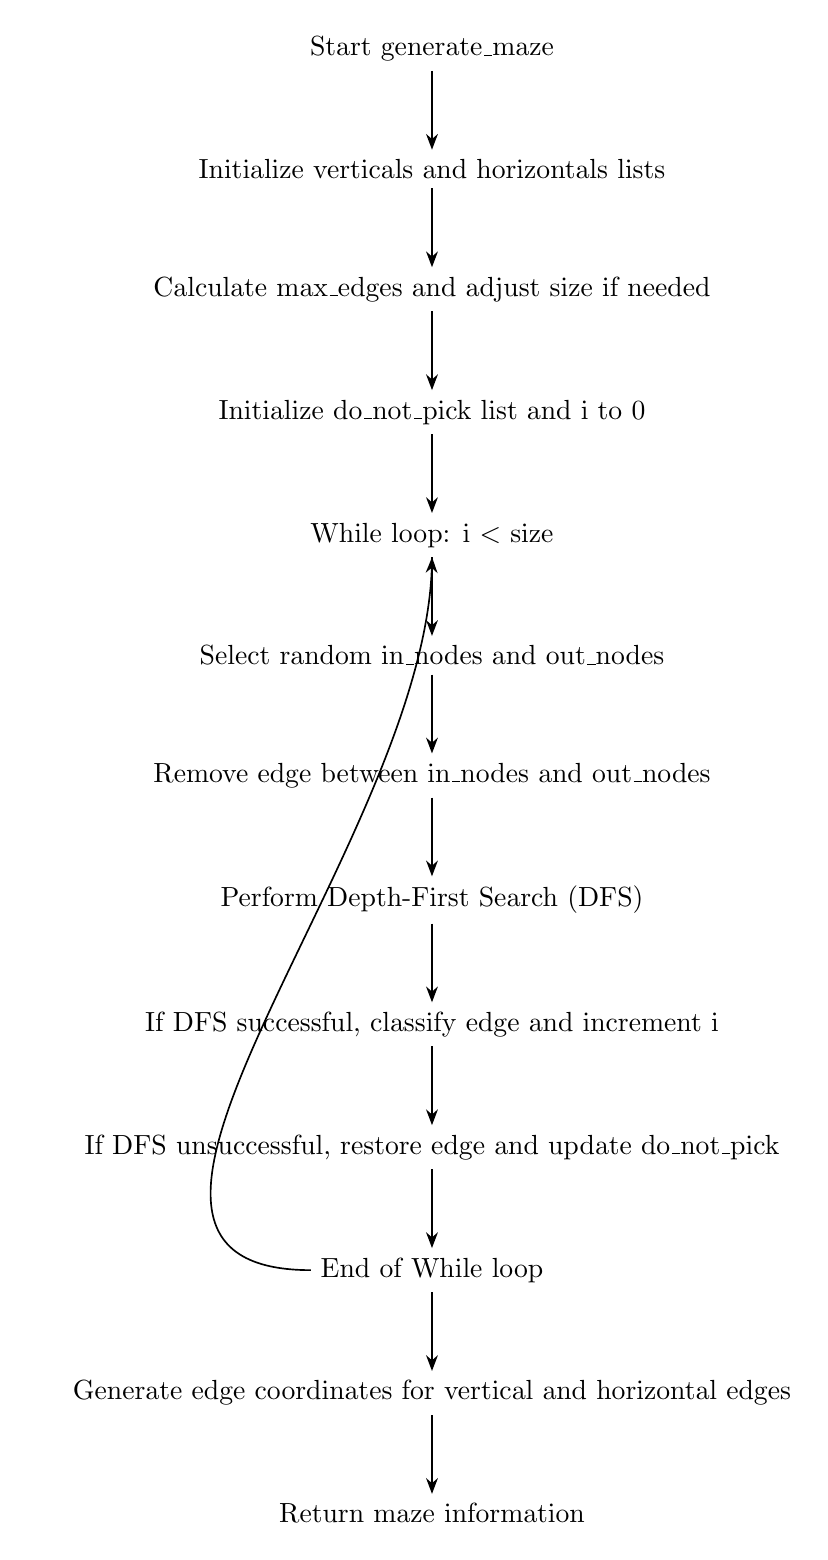
\begin{tikzpicture}[arj/.style={semithick,-Stealth[bend]}]
\path[start chain=D going below,nodes={on chain,join=by arj,align=center}]
    node{Start generate\_maze}
    node{Initialize verticals and horizontals lists}
    node{Calculate max\_edges and adjust size if needed}
    node{Initialize do\_not\_pick list and i to 0}
    node[alias=loop]{While loop: i $<$ size}
    node{Select random in\_nodes and out\_nodes}
    node{Remove edge between in\_nodes and out\_nodes}
    node[alias=dfs]{Perform Depth-First Search (DFS)}
    node{If DFS successful, classify edge and increment i}
    node{If DFS unsuccessful, restore edge and update do\_not\_pick}
    node[alias=end]{End of While loop}
    node{Generate edge coordinates for vertical and horizontal edges}
    node{Return maze information};
    
\draw[arj] (end) to[out=180,in=-90]  (loop);
\end{tikzpicture}
}
\caption{Flowchart of the generate\_maze Algorithm}
\label{fig:generate_maze_flowchart}
\end{figure}




\begin{figure}
\centering
\resizebox{0.4\textwidth}{!}{%
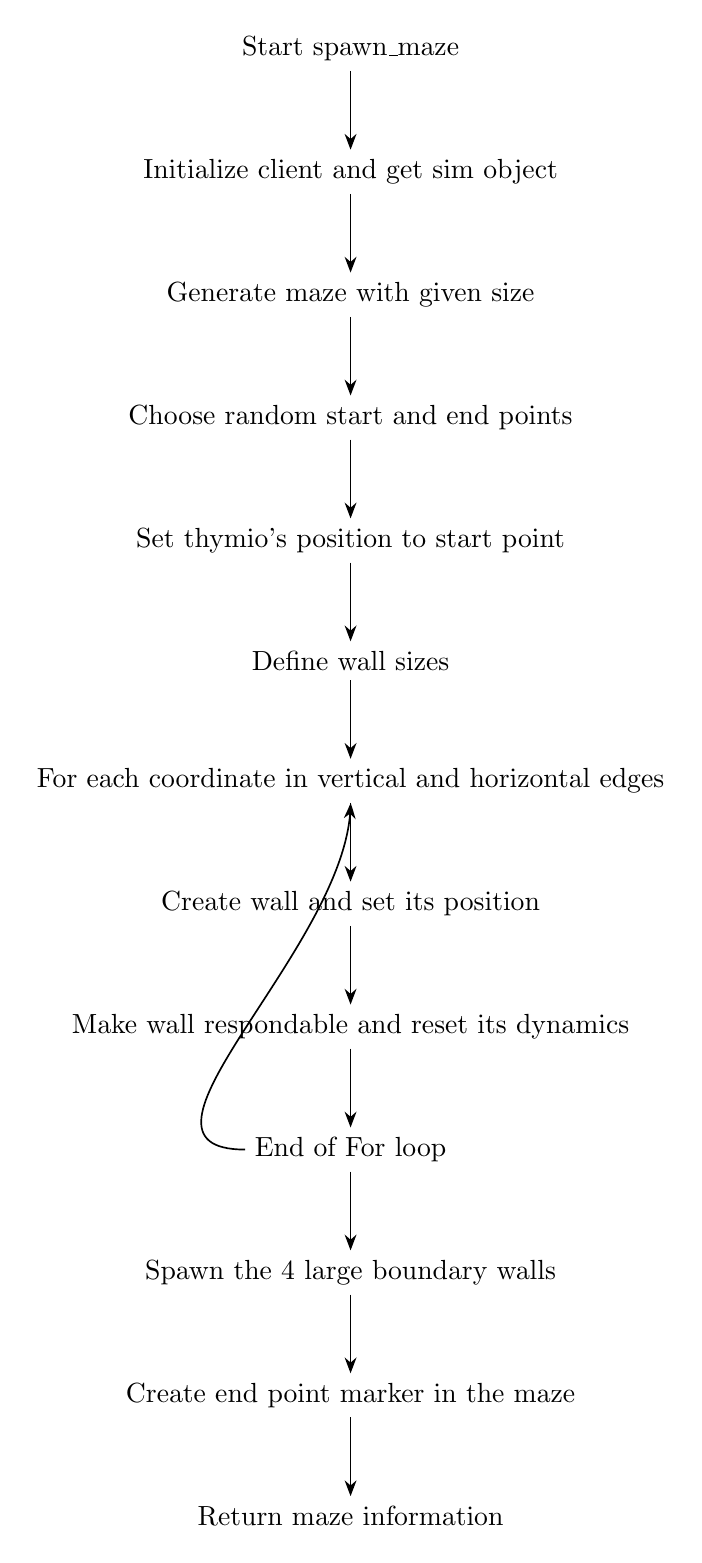
\begin{tikzpicture}[arj/.style={semithick,-Stealth[bend]}]
\path[start chain=D going below,nodes={on chain,join=by arj,align=center}]
    node{Start spawn\_maze}
    node{Initialize client and get sim object}
    node{Generate maze with given size}
    node{Choose random start and end points}
    node{Set thymio's position to start point}
    node{Define wall sizes}
    node[alias=loop1]{For each coordinate in vertical and horizontal edges}
    node{Create wall and set its position}
    node{Make wall respondable and reset its dynamics}
    node[alias=end1]{End of For loop}
    node{Spawn the 4 large boundary walls}
    node{Create end point marker in the maze}
    node{Return maze information};
    
\draw[arj] (end1) to[out=180,in=-90]  (loop1);
\end{tikzpicture}
}
\caption{Flowchart of the spawn\_maze Function}
\label{fig:spawn_maze_flowchart}
\end{figure}


\begin{figure}
\centering
\resizebox{0.5\textwidth}{!}{%
\begin{tikzpicture}[arj/.style={semithick,-Stealth[bend]}]
\path[start chain=D going below,nodes={on chain,join=by arj,align=center}]
    node{Start BiconnectedBFS}
    node{Initialize $to\_visit\_start$ and $to\_visit\_end$ queues}
    node{Start $thread\_start$ and $thread\_end$}
    node{Wait for both threads to finish}
    node[alias=q]{Is $meeting\_node$ None?}
    node[text=red]{Return None}
    node[alias=calc1]{Calculate path with $build\_path(parents\_start, parents\_end, meeting\_node)$};
    \path node[right=8em of calc1,text=green!70!black] (YES) {YES}
    (YES|-q) node (retPath) {Return calculated path};
    \draw[arj] (q) to[out=0,in=-90]  (YES);
    \draw[arj] (YES) to  (retPath);
\end{tikzpicture}
}
\caption{Flowchart of the BiconnectedBFS Algorithm}
\label{fig:biconnectedbfs_flowchart}
\end{figure}





\section{Explanation of the algorithms}

In the previous section, we explained how our algorithms work. In this section, we will explain the final algorithms in more detail.

% \begin{algorithm}
% \caption{Follow-right-wall Algorithm}\label{alg:follow-right-wall}
% \begin{algorithmic}[1]
% \Procedure{thymioController}{}
% \State `Initialize node parameters, publishers and subscribers`
% \While{`true`}
%     \State `Update sensor readings`
%     \If{`distance to endpoint $<$ threshold`}
%         \State `Stop and Exit`
%     \EndIf
%     \If{`no wall found yet`}
%         \State `Move and turn to find a wall`
%     \ElsIf{`no right wall and no front wall`}
%         \State `Move forward and turn right`
%     \ElsIf{`right wall and no front wall`}
%         \State `Adjust speed and direction based on right wall distance`
%     \ElsIf{`right wall and front wall`}
%         \State `Turn left`
%     \ElsIf{`front wall and no left and right wall`}
%         \State `Turn left`
%     \Else
%         \State `Move forward`
%     \EndIf
%     \State `Publish velocity commands`
% \EndWhile
% \EndProcedure
% \end{algorithmic}
% \end{algorithm}




\subsection{Maze Generation and Spawn}

A graph containing nodes and edges must be created to generate a maze. Using a depth-first search technique, we create the maze and spawned it into the CoppeliaSim environment.

The maze that the thymio must traverse in the CoppeliaSim is physically represented by obstacles (walls). The beginning and ending positions of the maze are chosen at random.

\subsection{Path Planning}

The goal of our path planning technique is to determine the most direct route from the maze's entrance to its exit. We developed appropriate path planning algorithms that takes into account the layout of the maze.

Concretely we implemented: BFS, DFS, BiconnectedBFS similar to RTT Biconnect) and a Dijkstra.

\subsection{Maze Navigation}

Without using the path planning we implemented follow-right-wall algorithm and a Runtime BFS algorithm without previous knowledge of the maze.

With the path planning we used the BFS biconnected algorithm to navigate the maze. When we move the thymio, we get its position from Coppelia and send it to its next position in an automatic way.

\section{Results}

Our project had encouraging outcomes. The produced mazes were successfully navigated by the thymio and also they where different for every run of coppelia. Also, we made work our path planning algorithm by successfully mapping coppelia to a graph and finding the shortest path between two nodes.

Our thymio was always able to complete the maze, independently of the maze's size or complexity in a reasonable amount of time depending of the algorithm, and the path planning algorithm was able to find the shortest path from the maze's entrance to its exit.

This is an example of a maze generated by our algorithm:


This is an example of the maze being spawned in coppelia:


This is an example of the thymio navigating the maze with the follow-right-wall algorithm:


This is an example of the thymio navigating the maze with the path planning algorithm:


This is an example of the thymio navigating the maze with the marzio real time algorithm:

\section{Errors}

The implementation of the project encountered a number of problems despite the thymio final effective navigation. The absence of collision detection with the maze walls was one of the key problems. The precision of the robot's movement and the efficiency of the path planning algorithm might both be impacted by the thymio's periodic collisions with the maze's walls.

The project's usage of out-of-date APIs was another problem. Even while these APIs were still usable, using them may cause issues later on since they might be altered or eliminated, which would perhaps cause our implementation's functionality to be broken. Later we discovered that have to use ZMQ Remote API instead of the legacy Remote API.

We also had many problems until we got the maze generation. We had to change the algorithm many times until we got it right. We also had to change the way we were spawning the maze in coppelia, because we were spawning the maze in the wrong way. We also had to change the way we were mapping the maze to a graph, because we were mapping it in the wrong way. We also had to change the way we were doing the path planning, because we were doing it in the wrong way. We also had to change the way we were navigating the maze, because we were navigating it in the wrong way. blablabla

\section{Conclusion}

In conclusion, our experiment proved the thymio's capacity to independently navigate a dynamic maze. The overall findings were encouraging despite a lot of implementation difficulties.

\end{document}
